\chapter{Digital Signal Processor}

%----------------------------------------------------------------------------------------
%	Section
%----------------------------------------------------------------------------------------

\section{ADSP-BF548 EZ-KIT Lite}

\subsection{Hardware Architecture}

\subsubsection{Audio Codec}
An Analog Devices AD1980 audio codec is the audio interface of the EZ-KIT Lite. The codec connects to multiple audio connectors (3.5 mm) which allow us to get audio in and out. These connectors can be easily found at the bottom left corner of the board.

\begin{figure}[H]
\centering
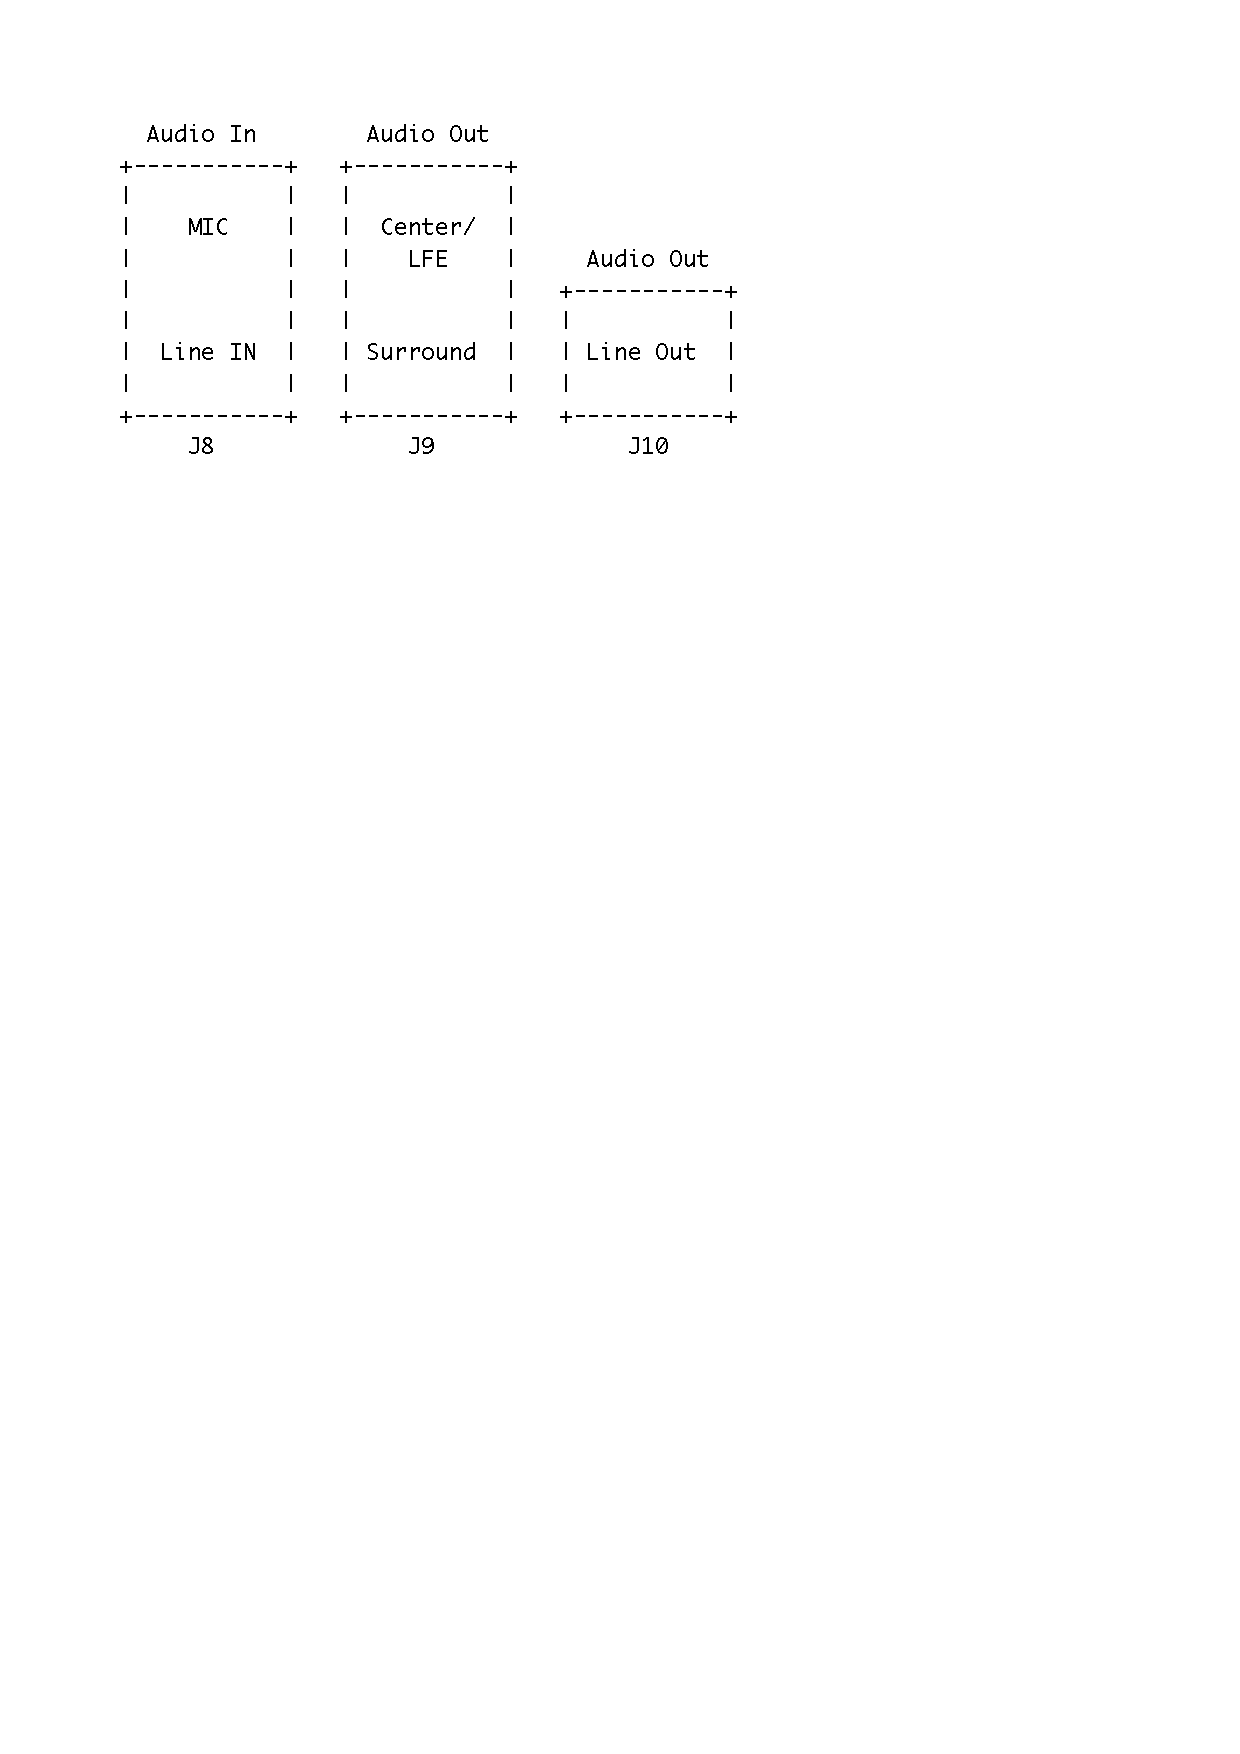
\includegraphics[width=3in]{ang/audio-connectors}
\caption{Audio Connectors}
\label{audio-connectors}
\end{figure}

Fig. \ref{audio-connectors} illustrates that the top location of \texttt{J8} is for a stereo microphone and the bottom location is for a stereo line in. According to Fig. \ref{AD1980-schematic}, the difference between MIC and LINE IN is signals via MIC will be pre-amplified. The preamp gain is collaboratively controlled by MIC Volume Register (\texttt{AD1980\_REG\_MIC\_VOL\_CTRL}) and Miscellaneous Control Bit Register (\texttt{AD1980\_REG\_MIC\_VOL\_CTRL}) \cite{AC97-codec}. In addition, it can be clearly seen that AD1980 can only sample 2 channels at any given moment due to the RECORD SELECTOR multiplexer. Thus, we decide to input noisy command and noise via the left / right channel of \texttt{MIC} respectively.

\begin{figure}[H]
\centering
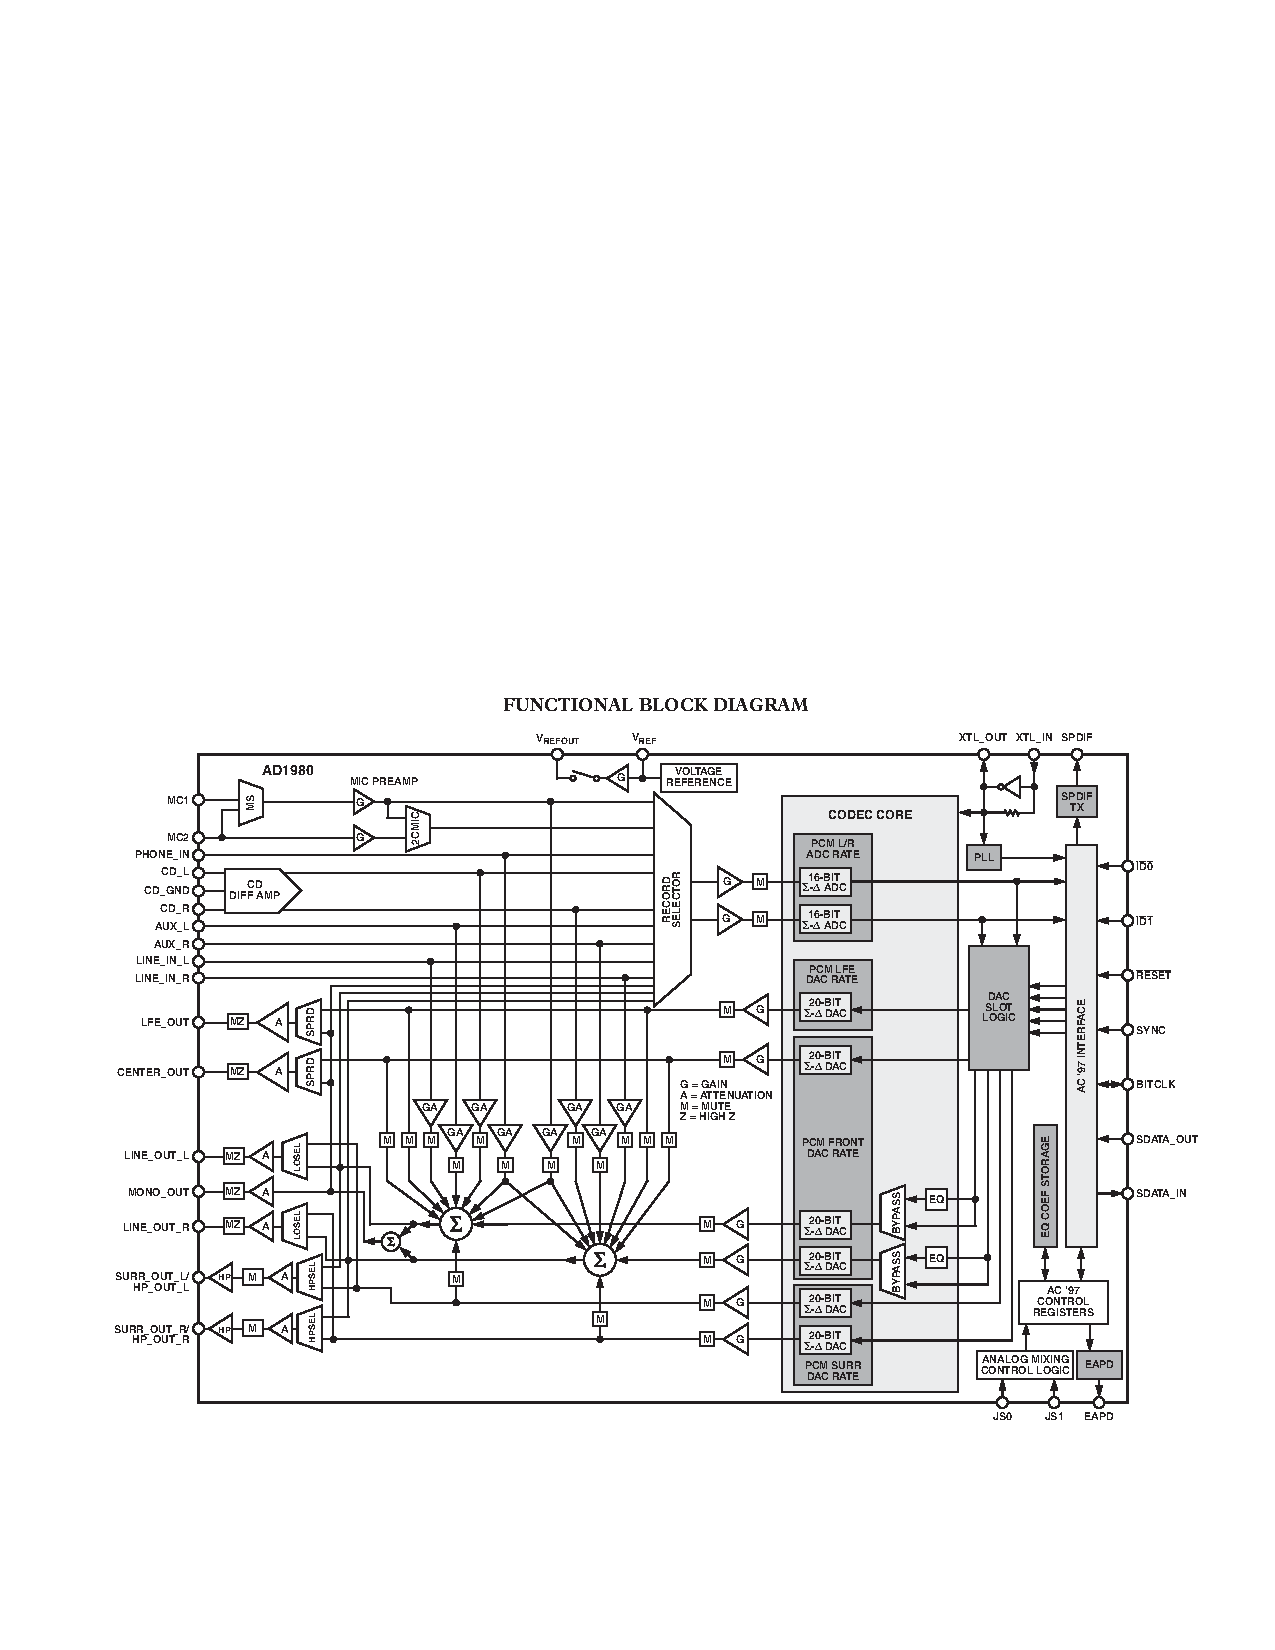
\includegraphics[width=6in]{ang/AD1980-schematic}
\caption{AD1980 Functional Block Diagram}
\label{AD1980-schematic}
\end{figure}

%--------------------------------------------

\subsubsection{Memory Hierarchy}
The ADSP-BF548 processor supports a hierarchy of three synchronous memories.\\

Internal L1 memory consists of two 32 KB data SRAM banks \cite{bf54x-hardware}. L1 memory is the highest-performing memory available to the Blackfin core and can be accessed at core clock speeds \cite{start-with-bf548}.\\

Internal L2 memory consists of a single 128 KB area of SRAM. L2 is slightly lower-performing than L1, requiring two core clock cycles for access. L2 provides more capacity accompanied by higher latency. \cite{start-with-bf548}\\

External memory is a 64 MB DDR SDRAM that exists external to the processor mounted on the DSP board. External memory operates synchronously with the system clock rather than the core clock, causing access time to SDRAM to be relatively slower than to L1 or L2 memory \cite{start-with-bf548}.

\subsection{Performance Tuning Guidelines}

%--------------------------------------------
%--------------------------------------------

\subsection{CrossCore Embedded Studio}

During ELEN90058 \textit{Signal Processing} and ELEN90052 \textit{Advanced Signal Processing} workshop sessions, we used CrossCore\textsuperscript{\textregistered} Embedded Studio to compile and debug code for Blackfin DSP board. Basing on Eclipse, CCES exploits the ecosystem of third-party tools already available to Eclipse developers. Thus, plenty of convenient functions such as plotting arrays of data are available to users \cite{erik-cces}\cite{cces-faq}. CCES could be an ideal substitution for VisualDSP++.\\

However, the AD1980 Audio Codec on ADSP-BF548 EZ-Kit Lite Board is not supported with CCES \cite{cces-ad1980}. Analog Devices engineer Craig Gilchrist explained in \textit{EngineerZone} support community that they do not have a driver for the AD1980 Codec with CCES. In addition, he recommended AD1836 Audio Codec instead \cite{BF548-BSP}.\\

Considering the project budget and potential risk, we eventually decided to stick on VisualDSP++ 5.1.2.

%----------------------------------------------------------------------------------------
%	Section
%----------------------------------------------------------------------------------------

\section{C Program}

\subsection{Audioloopback}

%--------------------------------------------
%--------------------------------------------

\subsection{Pre-emphasis}

It is easy to prove that filter characteristic represented by (\ref{shelving-filter}) will not change if coefficients $a_i$ and $b_i$ are uniformly scaled. Some pre-emphasis filter coefficients (\ref{shleving-coef}) are beyond the fractional data types domain $[-1, 1]$. Hence, the coefficients are scaled by $\lambda$ before converting them from \texttt{float} to \texttt{fract32}.\\

We choose $\lambda = \frac{1}{4}$ primarily because $\frac{1}{a_0} = \frac{1}{\lambda} = 4$ which is a power of 2. In terms of fixed-point data types, left shifting 2 bits is equivalent to multiplying by $\frac{1}{a_0} = 4$ but left shifting is more efficient. Besides, $\lambda = \frac{1}{2}$ is not small enough while $\lambda = \frac{1}{8}$ leads to loss in precision. $\forall a_i \in [-1, 1]$ and $\forall b_i \in [-1, 1]$ when $\lambda = \frac{1}{4}$.

\begin{align*}
&\begin{cases}
a_0 = \frac{1}{4} = 0.25\\
a_1 = \frac{-1.523796}{4} = -0.380949\\
a_2 = \frac{0.649345}{4} = 0.162336
\end{cases}
&\begin{cases}
b_0 = \frac{1.861856}{4} = 0.465464\\
b_1 = \frac{-3.102851}{4} = -0.775712\\
b_2 = \frac{1.366544}{4} = 0.341636
\end{cases}
\end{align*}

Filter coefficients are converted into \texttt{fract32} once by \texttt{calc\_shelving\_coef()} function when initializing the system. Finally, all computations in \texttt{pre\_emphasis()} function are fixed-point arithmetic.
